\chapter{A Conceptual Model of the Carbon Cycle}
\label{chapter:conceptual_carbon_cycle}
\graphicspath{{box_ocean/figs/}}

In \cref{chapter:global_bomb}, I showed that there were conditions under which the climate was unstable,
driven by an instability in the terrestrial carbon cycle. In that chapter I found that the effects of
the biogeochemical feedback were small at the global scale. I also used a parameter $\chi_0$ to model the ocean,
which is a obvious simplification.

In this chapter then, I will construct a model of the climate-carbon system which is analytically tractable
with a dynamical ocean component but neglects the role of biochemical heating.

\section{Background}

\subsection{Climate Response to Radiative Forcing}
When certain gases, known as Greenhouse Gases, are emitted into the atmosphere they can affect global temperatures.
They do this by absorbing infrared radiation emitted by the Earth's surface and re-radiating it to space at a lower temperature.
The effect of this is that less energy is radiated away to space than it did before the emission of greenhouse gases. To be in
equilibrium, the energy received from the Sun must equal the energy radiated to space by the Earth. As less radiation is now
emitted to space the Earth's climate responds to restore equilibrium. It does this by warming up to increase the amount it
radiates to restore equilibrium.

The amount that a greenhouse gas decreases the outgoing radiation to space by is known as its radiative forcing. If $T$ is
the global mean temperature and $N(T)$ is the net radiation received by the Earth (in equilibrium $N$ is zero) then for a small
radiative forcing $\Delta N$ the change in global mean temperatures is
\begin{equation}
  \label{eq:response_to_radiative_forcing}
  \Delta N = \pdv{N}{T} \Delta T.
\end{equation}
The quantity
\begin{equation}
  \label{eq:climate_sensitivity}
  \lambda = -\pdv{N}{T}
\end{equation}
known as the \emph{climate sensitivity} determines the amount of warming experienced for a given radiative forcing. This quantity is measured
in units \si{\watt\per\square\meter\per\kelvin} but it has become common to discuss $\lambda$ in terms of a given radiative forcing, $Q_{2\times}$,
the radiative forcing due to doubling the concentration of $\ce{CO2}$ in the atmosphere, giving rise to
\begin{equation}
  \label{eq:definition_of_ECS}
  \mathrm{ECS} = \frac{Q_{2\times}}{\lambda}
\end{equation}
known as \emph{Equilibrium Climate Sensitivity} which is measured in \si{\kelvin}.

Implicit in this definition is the idea that $Q_{2\times}$ is well defined. It is an empirical fact that over a range of concentrations the radiative forcing
of $\ce{CO2}$ varies with the logarithm of its concentration, and so the notion of a radiative forcing due to doubling is well defined. It is also usually assumed that
$\mathrm{ECS}$ is a constant independent of background climate state. Whilst this appears to be a good approximation, it has been challenged.

The value of $\mathrm{ECS}$ is uncertain. State of the art climate models (CMIP6) do not agree on its value, and give a range of \SIrange{1.8}{5.6}{\kelvin}, which represents an
increase in uncertainty from CMIP5. However, these estimates should be combined with other observational estimates as well as paleoclimate records. Doing this sort of
analysis leads the IPCC to conclude that the best estimate of $\mathrm{ECS}$ is \SI{3.0}{\kelvin} with a likely range of \SIrange{2.5}{4.0}{\kelvin}.

\subsection{Terrestrial Carbon Cycle Response to \ce{CO2}}
Whilst the above discussion of $\mathrm{ECS}$ treats the amount of $\ce{CO2}$ in the atmosphere as a given quantity, in reality it is also affected by the climate
system, which determines the fluxes of carbon into and out of the atmosphere through biogeochemical cycles.

On human-relevant timescales, these fluxes are controlled by terrestrial and ocean processes. The terrestrial part of the carbon cycle is controlled by the biosphere.
Carbon enters the biosphere through photosynthesis and leaves via respiration. Respiration can be subdivided into \emph{autotrophic} and \emph{heterotrophic}.
These relate to respiration done by plants (which produce their own food which hence the name \emph{auto}troph) and non-plants respectively. Heterotrophic respiration
is primarily performed by soil microbial communities which decompose the organic matter deposited into the soil from plants.

This means that the net carbon flux into the biosphere due to plants called \emph{Net Primary Productivity} (NPP) is given by the difference between photosynthesis and
autotrophic respiration. The overall carbon flux between the land and the atmosphere is therefore the difference between NPP and heterotrophic respiration. There are two key feedbacks
on NPP and heterotrophic respiration related to elevated \ce{CO2} levels that I will discuss.

Firstly, increasing $\ce{CO2}$ increases the amount of carbon available for plants to photosynthesise. This means that if a plant's photosynthetic activity is limit by
$\ce{CO2}$ (as opposed to light or nutrients) then increases \ce{CO2} will increase NPP\@. This \emph{\ce{CO2} fertilisation effect} has been detected. It acts as a negative feedback
on global warming as it tends to decrease the amount of \ce{CO2} in the atmosphere by increasing photosynthesis. This feedback is expected to decrease with increased $\ce{CO2}$ as
fewer plants become limited by available carbon.

Secondly, the decomposition of organic matter is a biochemical process that depends on temperature. In particular, increasing the temperature of the decomposition reaction
will increase the rate of this reaction. Hence as $\ce{CO2}$ has a warming effect the amount of respiration will increase. This means there will be a larger flux of carbon to the
atmosphere and so this is a positive feedback. Many biological reactions are assumed to depend exponentially on temperature, increasing in rate by a factor $Q_{10}$ for every
\SI{10}{\kelvin} of warming. It is generally thought that $Q_{10} \approx 2$.

The net effect of these two feedbacks is that the terrestrial response to \ce{CO2} is uncertain as the sign of the response depends on the relative magnitude of these effects. Overall it
is thought that the heterotrophic respiration effect is larger, which leads to a net positive feedback on the climate system.

\subsection{Potential For Runaway}
Combining these two sensitivities gives the potential for a runaway effect. Consider the following situation. Suppose some carbon is transferred from the land to the atmosphere. Then the globe
will warm. As the feedback from the land is positive more carbon will be released into the atmosphere leading to further warming and more carbon released. This cycle could continue until all the
carbon from the land has been released into the atmosphere. The fact that there is carbon on land therefore tells us something about the magnitudes of the land carbon feedback and the climate sensitivity.
To make progress analysing this we must include the effect of the other store of carbon: the ocean.

\section{A Climate-Carbon Cycle model using IMOGEN as the Ocean Component}
\subsection{IMOGEN description}
The land surface model JULES is often used in conjunction with IMOGEN \parencite{Huntingford2004,Huntingford2010} which is a model that `closes' the carbon cycle in that it provides
an atmospheric and oceanic response to changes in terrestrial carbon. For the purposes of this chapter, we will isolate the ocean component of IMOGEN. The ocean component is based on the
model of \cite{Joos1996} which represents ocean carbon in terms of an impulse response to atmospheric \ce{CO2}.

It calculates the changes in dissolved inorganic carbon in the surface water as
\begin{equation}
  \label{eq:imogen_upper_ocean_carbon}
  \delta \Sigma \ce{CO2} = \int_0^{t} F_{a}(t-s)G_{I}(s)\dd{s}.
\end{equation}
where $F_a$ is the atmosphere to ocean flux of carbon and $G_I$ is IMOGEN's impulse-response function. This function is defined as
\begin{equation}
  \label{eq:imogen_impulse_response}
  G_I(t) =
  \begin{cases}
    1 - 2.2617t + 14.002t^2 - 48.770t^3 & t \leq \SI{1}{\year} \\
    f_0 + \sum_{i=1}^{5} f_i e^{-t/\tau_i} & t > \SI{1}{\year}
  \end{cases}
\end{equation}
where $f_0=0.014819,f_1 = 0.70367,f_2=0.24966,f_3=0.066485,f_4 = 0.038344,f_5=0.019439$ and $\tau_1= 0.70177,\tau_2 = 2.3488,\tau_3=15.281,\tau_4 = 65.359,\tau_5 = 347.55$.
The carbon flux is given by
\begin{equation}
  \label{eq:imogen_ocean_atmosphere_flux}
  F(t) = k \left(\Delta C_a - \Delta C_o\right)
\end{equation}
where $\Delta C_a$ and $\Delta C_o$ are the perturbations in atmospheric and ocean carbon. To take into account ocean temperature feedbacks on the ocean carbon cycle $\Delta C_o$ and
$\delta \Sigma \ce{CO2}$ are related by
\begin{equation}
  \label{eq:imogen_temp_feedback}
  \Delta C_o = g(T_o,\delta \Sigma \ce{CO2})e^{0.0423\delta T_o}
\end{equation}
where $T_o$ is the initial ocean temperature, $\delta T_o$ is the change in ocean temperature and $g$ is a quintic polynomial in $\delta \Sigma \ce{CO2}$ whose coefficents depend on $T_o$.
\subsection{Terrestrial Carbon Cycle}
The total avaliable carbon is a constant given by $\mathcal{C}  = C_s + C_a + C_o$ where $C_s$ is the soil carbon, $C_a$ is the atmospheric carbon  and $C_o$ is the ocean carbon.
Therefore to close the system only the land carbon dynamics need to be set, with the dynamics of atmospheric carbon being set by this conservation law.

The change in soil carbon is given by the difference between net primary productivity and heterotrophic respiration. Heterotrophic
respiration has the following form:
\begin{equation}
  \label{eq:heterotrophic_respiration}
  R_h = r_0 C_s Q_{10}^{T_a/10} = r_0 C_s e^{\alpha T_a}
\end{equation}
where $T_a$ is the change in atmospheric temperature, $r_0$ is a reference respiration level and $\alpha = 0.1\log Q_{10}$ is the strength of the temperature feedback.

It is assumed that $T_a$ depends logarithmically on temperature
\begin{equation}
  \label{eq:air_temperature}
  T_a = \frac{S}{\log 2} \log \frac{C_a}{C_{a0}}
\end{equation}
where $C_{a0}$ is a reference \ce{CO2} level, set at \SI{589}{\peta\gram\carbon}. The parameter $S$ is a land-weighted climate sensitivity. This can be combined \cref{eq:heterotrophic_respiration}
to give
\begin{equation}
  \label{eq:heterotrophic_respiration_combined}
  R_h = r_0 C_s \left( \frac{C_a}{C_{a0}}\right)^{\mu}
\end{equation}
where
\begin{equation}
  \label{eq:mu}
  \mu = \frac{1}{\log 2} \alpha S.
\end{equation}


Following \cite{Cox2006}, net primary productivity is modelled as
\begin{equation}
  \label{eq:npp}
  \Pi(C_a) = \Pi_{\infty}\frac{C_a}{C_a + C_{1/2}},
\end{equation}
which is an increasing function of \ce{CO2} that saturates for $C_a \gg C_{1/2}$. Unless otherwise stated, $C_{1/2} = \SI{280}{\ppm}$, which is compatible with other estimates
\parencite{KolbySmith2016,Wenzel2016}. This parameter controls the strength of the \ce{CO2} fertilisation feedback. \Cref{eq:npp} assumes that net primary productivity depends only
on \ce{CO2}. Allowing for other factors like nitrogen limitation would act to reduce the effective $C_{1/2}$ value. $\Pi_{\infty}$ is set so that $\Pi(C_{a0})$ is the preindustrial
level of net primary productivity \SI{55}{\peta\gram\carbon\per\year}.

Putting this all together leads to the following set of coupled differential equations:
\begin{subequations}
  \label{eq:imogen_deterministic}
  \begin{align}
    \dv{C_s}{t}     &= \Pi(C_a) - C_s r_0 \left(\frac{C_a}{C_{a0}}\right)^\mu \\
    \dv{C_o}{t}     &= \mathrm{IMOGEN}(C_a,T_o,C_o) \\
    C_a             &= \mathcal{C} - C_s - C_o \\
    T_o             &= \frac{1}{\nu}\frac{S}{\log 2}\log \frac{C_a}{C_{a0}}
  \end{align}
\end{subequations}
where $T_o$ is the ocean temperature which is related to the land temperature by the factor $\nu = 1.45$. Note that $S$ and $Q_{10}$ (through $\mu$) appear separately in this equation,
so both parameters will affect the bifurcation point.

Note that there is an equilibrium at $C_a = C_{a0}$, $C_s = C_{s0} = \Pi(C_{a0})/r_0$, $C_o = 0$, $T_o = 0$, corresponding to the preindustrial equilibrium, which has been stable over the
holocene.

\subsection{Bifurcations in IMOGEN}
\Cref{eq:imogen_deterministic} is solved for a range of values of $S$ with $Q_{10} = 2$. The system was initilised close to equilibrium and then allowed to equilibriate over 5000 years.
The results for atmospheric carbon are plotted in \cref{fig:imogen_trajectories}. For values of $S$ between \SIrange{10}{11}{\kelvin} there appears to be a Hopf bifurcation which results
in osciallatory behaviour. 
\begin{figure}
  \centering
  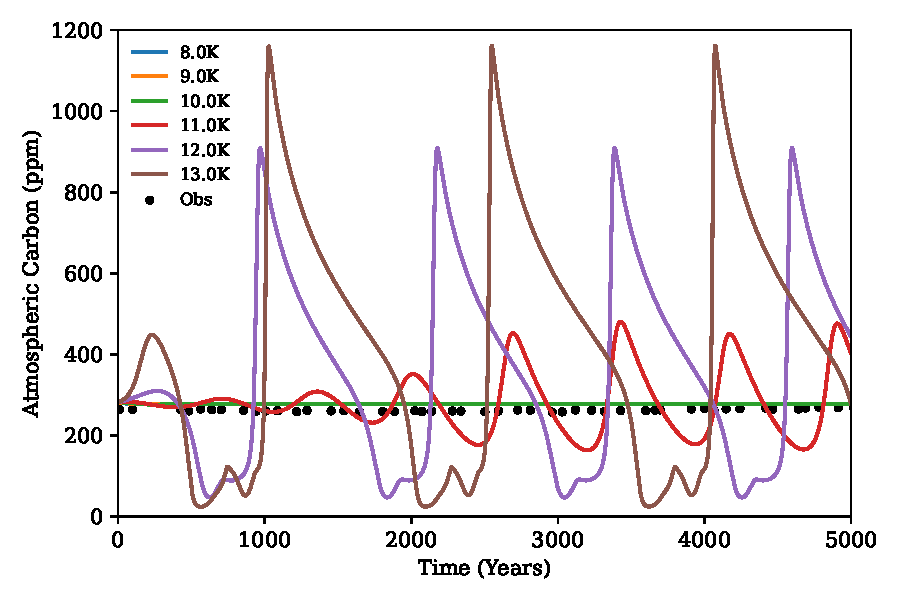
\includegraphics[width=\textwidth,keepaspectratio]{imogen_traj}
  \caption{Trajectories for IMOGEN, assuming $Q_{10} = 2$}
  \label{fig:imogen_trajectories}
\end{figure}

To be more complete, I use this IMOGEN model to estimate the critical $S$ as a function of $Q_{10}$ and $C_{1/2}$, the parameter that controls the \ce{CO2} fertilisation effect. This
is plotted in \cref{fig:imogen_bifurcation_plane}.

\begin{figure}
  \centering
  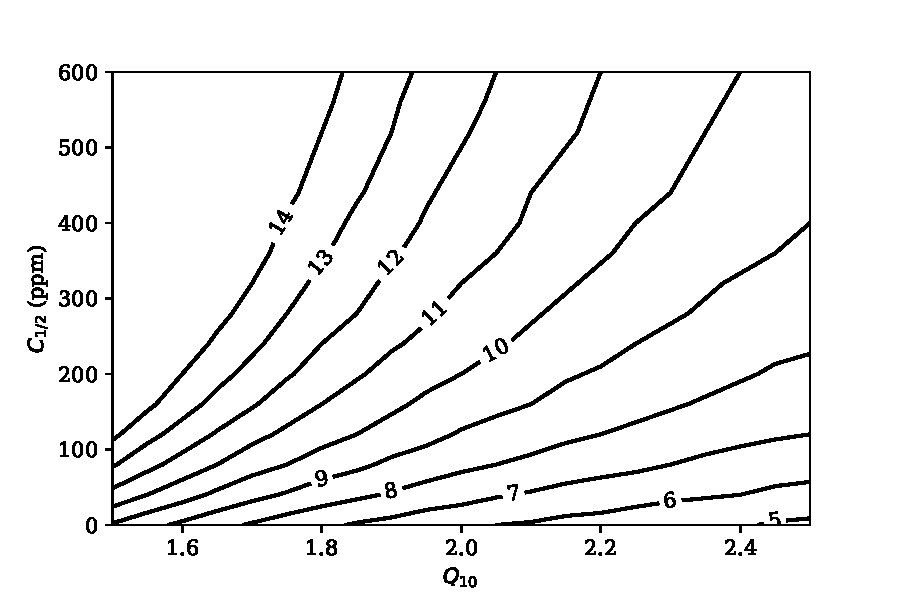
\includegraphics[keepaspectratio,width=\textwidth]{imogen_critical_S_Q10_ca05}
  \caption{Values of $S$ at the bifurcation point as a function of \ce{CO2} fertilisation and the strength of respiration feedback}
  \label{fig:imogen_bifurcation_plane}
\end{figure}

As some CMIP6 models have an $S \approx\SI{9}{K}$ this does impose limits on the strength of their carbon cycle feedback. Furthermore, because some models are
near this bifurcation point, they will be subject to critical slowing down and this will affect their variability, even if they are in the non-oscialltory branch of the carbon cycle.


\section{Ocean Model}
I will neglect temperature and chemical feedbacks on the ocean response and assume it behaves linearly to elevated \ce{CO2} levels. I will further assume that the ocean carbon carbon uptake
can be viewed as $N$ non-interacting boxes which each respond over a timescale $\tau_i$ where $i$ indexes the boxes. A fraction $f_i$ of the total carbon
flux will enter the $i$th box. I will give a post-hoc justification for this in that this model can capture the observed carbon uptake of the oceans since pre-industrial times and
will qualitatively reproduce the results of a more complex ocean model. The model I introduce here has the advantage that it can be treated analytically.

The change in carbon stored in the $i$th box, $C_i$, is given by
\begin{equation}
  \label{eq:ocean_box_i}
  \dv{C_i}{t} = f_ik \Delta C_a(t) - \frac{C_i}{\tau_i},
\end{equation}
where $k=\SI{0.2}{\per\year}$ gives the timescale of the ocean uptake and $\Delta C_a$ is the change in atmospheric carbon from its equilibrium value.

For a given $C_a(t)$ \cref{eq:ocean_box_i} can be solved in quadratures to give
\begin{equation}
  \label{eq:solution_for_box_i}
  C_i(t) = \int_0^t f_ik e^{-s/\tau_i} \Delta C_a(t - u) \dd{u},
\end{equation}
if $C_i(0) = 0$.


The overall ocean response is therefore
\begin{equation}
  \label{eq:ocean_response}
  \Delta C_o(t) = \sum_{i=1}^N \int_0^t f_ik e^{-s/\tau_i} \Delta C_a(t - s) \dd{s}.
\end{equation}
or
\begin{equation}
  \label{eq:ocean_response_in_terms_of_G}
  \Delta C_o(t) = \int_0^t G(s) \Delta C_a(t-s) \dd{s}
\end{equation}
where
\begin{equation}
  \label{eq:ocean_greens_function}
  G(t) = \sum_{i=1}^{N} f_ik e^{-t/\tau_i}
\end{equation}
is the impulse response function for the uptake of ocean carbon.

\subsection{Parameter Estimation}
\Cref{eq:ocean_response} can then be fitted to observed changes in ocean carbon\todo{give details} to estimate the
parameters $f_i$ and $\tau_i$. I will do this for a one box model, in which only $\tau_1$ needs to be estimated and
for a two box model where $\tau_1$,$\tau_2$ and $f_1$ must be estimated. The quantity $f_2$ is determined by the requirement that $f_1 + f_2 = 1$.
\begin{table}
  \centering
  \begin{tabular}{@{}lll@{}}
    \toprule
    \multicolumn{1}{c}{Parameter} & \multicolumn{2}{c}{Estimated Quantity} \\
    \cmidrule{2-3}
                                  & One Box         & Two Box              \\
    \midrule
    $\tau_1$                      & \SI{3.7}{\year} & \SI{0.5}{\year}      \\
    $\tau_2$                      &                 & \SI{124}{\year}      \\
    $f_1$                         & $1$             & $0.9$                \\
    $f_2$                         & $0$             & $0.1$                \\
    \bottomrule
  \end{tabular}
  \caption{Parameter Estimates for one and two box ocean models}
  \label{tab:one_and_two_box_parameters}
\end{table}
Taking ocean carbon sink data and atmospheric \ce{CO2} data from the global carbon budget from the year 1781 onwards (which is
when the ocean sink data is available) and assuming that ocean carbon and atmospheric carbon is in equilibrium in this year I perform a
least squares fit to the one and two box models giving the parameter estimates shown in \cref{tab:one_and_two_box_parameters}.

\begin{figure}
  \centering
  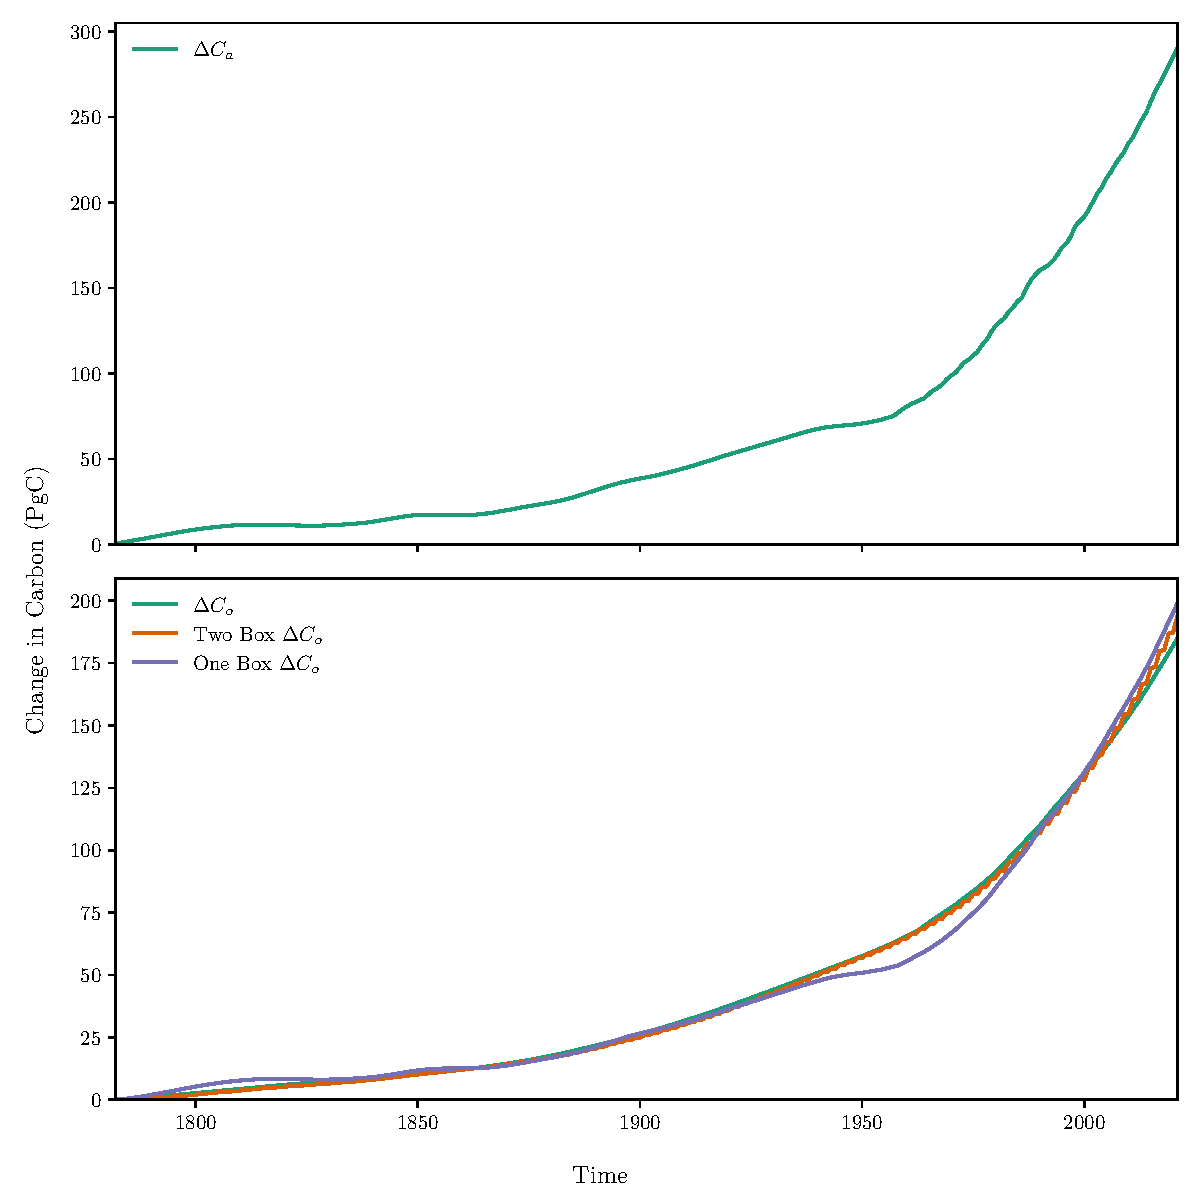
\includegraphics[keepaspectratio,width=\textwidth]{gcb_ocean_atmosphere_boxes}
  \caption{The reconstructed ocean uptake using the one and two box models, with parameters from \cref{tab:one_and_two_box_parameters}}
  \label{fig:fits_from_one_and_two}
\end{figure}


These fits are plotted in \cref{fig:fits_from_one_and_two}. It can be seen that both one and two box models do a reasonable job in capturing the
historical record of ocean carbon uptake. However the two box model does substantially better.



\section{One Box Ocean}
Although the two-box ocean model does better than the one box ocean model in fitting the observed carbon sink, the one box model is simpler
and more easily analysable. Therefore as a warm up, I will analyse the stability of the carbon cycle assuming a one box ocean.

I assume Net Primary Productivity is a function of the atmospheric carbon only that saturates at high \ce{CO2}, having the form
\begin{equation}
  \label{eq:npp}
  \Pi(C_a) = \Pi_{\infty}\frac{C_a}{C_a + C_{1/2}}.
\end{equation}
I model heterotrophic respiration as having a $Q_{10}$ temperature dependence:
$R_h = r_0 C_s e^{\alpha T}$ where $r_0$ is the specific respiration, $\alpha = \log \left( Q_{10} \right)/10$ and $C_s$ is the soil carbon. The global temperature anomaly, $T$,
is set assuming a logarithmic dependence on atmospheric \ce{CO2} giving $T = S \log \left(C_a / C_{a0}\right)/\log 2$ where $C_a$ is the atmospheric carbon, $C_{a0}$ is a reference level of
atmospheric carbon which I take as corresponding to the pre-industrial state, which I assume is stable. The parameter $S$ is related to the climate sensitivity, although it is land-weighted.
I set $r_0 = \Pi(C_{a0})/C_{s0}$ where $C_{s0}$ is a reference level of soil carbon, set to the pre-industrial level.  

The ocean carbon dynamics are set by the one box model described in \cref{eq:ocean_box_i} and the level of atmospheric carbon is set through conservation of carbon, namely $\mathcal{C} = C_a + C_s + C_o$,
where the total carbon in the atmosphere-land-ocean system to $\mathcal{C}$.

These assumptions give rise to the following set of equations.
\begin{subequations}
  \label{eq:one_box_ocean}
  \begin{align}
    \dv{C_s}{t} &= \Pi(C_a) - r_0 C_s \left(\frac{C_a}{C_{a0}}\right)^{\mu} \\
    \dv{C_o}{t} &= k(C_a - C_{a0}) - \frac{C_o}{\tau} \\
    C_a &= \mathcal{C} - C_s - C_o.
\end{align}
\end{subequations}
The parameter $\mu = \alpha S / \log 2$ will be the control parameter that determines the stability of the system.
Note that there is a fixed point at $C_a = C_{a0}$, $C_o = 0$ and $C_s = C_{s0}$. I am interested in its stability.
\subsection{The Stability of a fixed point}
Here I give a summary of the conditions for an equilibrium to stable. Let
\begin{equation}
  \label{eq:generic_system}
  \dv{\bm{x}}{t} = f(\bm{x})
\end{equation}
with $\bm{x} \in \mathbb{R}^n$ and $f: \mathbb{R}^n \rightarrow \mathbb{R}^n$. Suppose there is a fixed point at $\bm{x}^*$, so $f(\bm{x}^*) = \bm{0}$. Then linearising around this
fixed point gives
\begin{equation}
  \label{eq:generic_system_linearised}
  \dv{\bm{y}}{t} = J\bm{y}
\end{equation}
where $\bm{y} = \bm{x} - \bm{x}^*$ and $J$ is the Jacobian defined by
\begin{equation}
  \label{eq:generic_jacobian}
  J_{ij} = \pdv{f_i}{x_j}.
\end{equation}
This fixed point is stable if no eigenvalues of $J$, denoted $\gamma$, have positive real part.
\subsection{Stability of One Box}
The Jacobian of \cref{eq:one_box_ocean} is given by
\begin{equation}
  \label{eq:jacobian_of_one_box}
    \bm{J} = 
    \begin{pmatrix}
    r_0 \left( \mu \frac{C_{s0}}{C_{a0}} - 1\right) - \Pi'(C_{a0}) & 
    \mu \frac{C_{s0}}{C_{a0}} - \Pi'(C_{a0}) \\
    -k & -k - \frac{1}{\tau}
    \end{pmatrix}
  \end{equation}
where $\Pi'(C_a)$ denotes there derivative of NPP with respect to atmospheric carbon.
  
To finds the eigenvalues of the Jacobian, I must solve the characteristic polynomial $\det(\bm{J} - \gamma \bm{I})$ = 0, where $\gamma$ is an eigenvalue.

This equation is quadratic and therefore has two roots. Solving it leads to a solution of the form:
\begin{equation}
  \label{eq:eigenvalues_of_one_box_jac}
  \gamma_{\pm} = \frac{B \pm \sqrt{\Delta}}{2\tau C_{a0}}
\end{equation}
where
\begin{equation}
  \label{eq:B_in_one_box}
  B = -k \tau  C_{a0}-\Pi'(C_{a0}) \tau  C_{a0}-r_0 \tau  C_{a0}-C_{a0}+\mu  \Pi_0 \tau
\end{equation}
and
\begin{equation}
  \label{eq:discriminant_from_one_box}
  \Delta = \left(k \tau  C_{a0} +\Pi'\tau  C_{a0}+r_0 \tau  C_{a0}+C_{a0}-\mu  \Pi_0 \tau \right)^2-4 \left(k r_0 \tau ^2 C_{a0}^2+\Pi' \tau  C_{a0}^2-\mu  \Pi_0 \tau  C_{a0} +r_0 \tau  C_{a0}^2\right)
\end{equation}
is the discriminant. I have used $\Pi_0 = r_0 C_{s0}$.

The stability of this system is governed by $\Re \gamma$. This number is controlled by the sign of $\Delta$. If $\Delta > 0$, then $\Re \gamma = \gamma$, but if $\Delta < 0$, then
$\Re \gamma = B / 2\tau C_{a0}$. 

\subsection{Real Eigenvalues}
If $\tau < 1/r_0$ then $\Delta > 0$ for all values of $\mu$. As $1/r_0 \approx 30$ year this situation represents a relatively fast ocean response.
Under this assumption, it turns out that $\gamma_+ > 0$ when
\begin{equation}
  \label{eq:instability_condition_one_box_fast}
  \mu^* = \frac{C_{a0}}{C_{s0}} + \frac{C_{a0}}{\Pi_0} \dv{\Pi}{C_a} + \frac{C_{a0}}{C_{s0}} k\tau.
\end{equation}
It is interesting to compare this to the condition given in \cref{eq:mu_infinity}. If the parameter $\chi_0$ is introduced and set to $\chi_0 = k \tau$.
then \cref{eq:instability_condition_one_box_fast} is identical to \cref{eq:mu_infinity}. This gives an interpretation to $\chi_0$ as the ratio of the timescale of the ocean carbon flux
to the timescale of its response. Previously, $\chi_0$ was interpreted as a fraction. This can be done only if $\tau < 1/k = \SI{5}{\year}$.
\begin{figure}
  \centering
  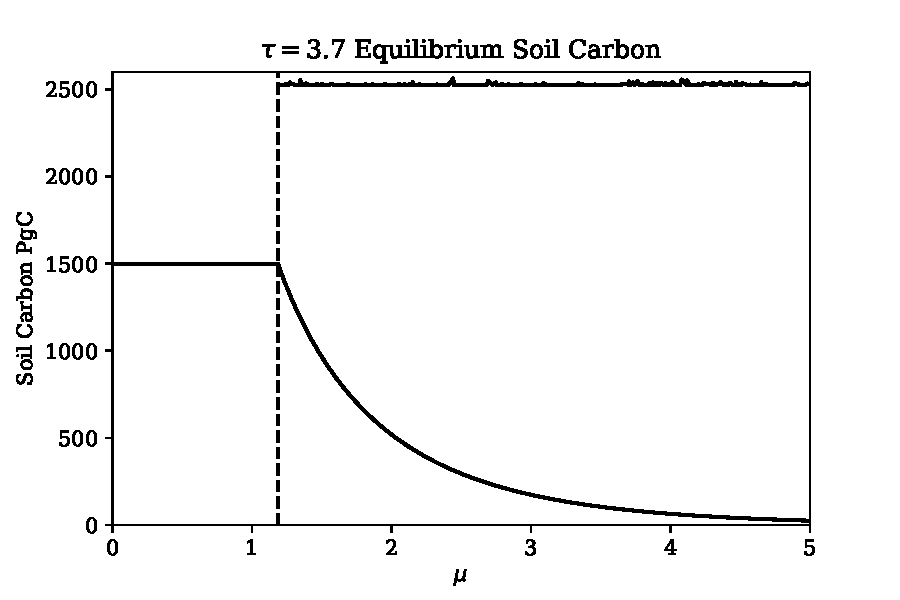
\includegraphics[keepaspectratio,width=\textwidth]{one_box_model_soil_carbon_equilibrium_tau_3.7}
  \caption{Equilibrium Soil Carbon level as a function of $\mu$ for a fast ocean response}
  \label{fig:fast_response_bf_diagram}
\end{figure}

The system \cref{eq:one_box_ocean} is integrated to equilibrium and the equilibria are plotted as a function of $\mu$ in \cref{fig:fast_response_bf_diagram}.
I set $C_{1/2} = \SI{593.6}{\peta\g\carbon}$ and chose $\Pi_{\infty}$ so that $\Pi(C_{a0}) = \SI{55}{\peta\g\carbon\per\year}$. In this case, $\tau = \SI{3.7}{\year}$.
The dashed line represents the position
of the analytically calculated bifurcation point. It can been seen that the agreement is good, and that this is a transcritical bifurcation.
To the extent that this model is valid, this imposes an upper limit on the possible value of $\mu$ given
the observed stability of the pre-industrial climate.

\subsection{Complex Eigenvalues}
In the case where the ocean timescale is larger than $1/r_0$, then $\Delta < 0$. This means if the ocean response is considered to have a long timescale,
the stability of the system is given by the sign of $B$.

The value of $B$ will become positive when $\mu$ exceeds the following threshold:
\begin{equation}
  \label{eq:instability_condition_one_box_slow}
  \mu^* =\frac{C_{a0}}{C_{s0}} + \frac{C_{a0}}{\Pi_0} \dv{\Pi}{C_a} + \frac{C_{a0}}{C_{s0}} k\tau\left(
     1 + \frac{1}{k\tau}
  \right) \frac{1}{r_0\tau}
\end{equation}
This is similar to the conditions derived in \cref{eq:mu_infinity,eq:instability_condition_one_box_fast} except now $\chi_0 = k\tau\left(1 + \frac{1}{k\tau} \right) \frac{1}{r_0\tau} \approx \tau/r_0$
where the approximation assumes $k \gg r_0$. This means the ``fraction absorbed by the oceans'' is now controlled by the ratio of the timescale of the oceans as well as the turnover time of the soil.
Furthermore we are assuming that $\tau r_0 > 1$ in this case and so $\chi_0 > 1$ so it loses its interpretation as a fraction of carbon absorbed.


In addition, because $\gamma$ is complex, this bifurcation occurs when the complex conjugate eigenvalue pair crosses the imaginary axis. This means this bifurcation is
a Hopf bifurcation rather than a transcritical bifurcation.
\begin{figure}
  \centering
  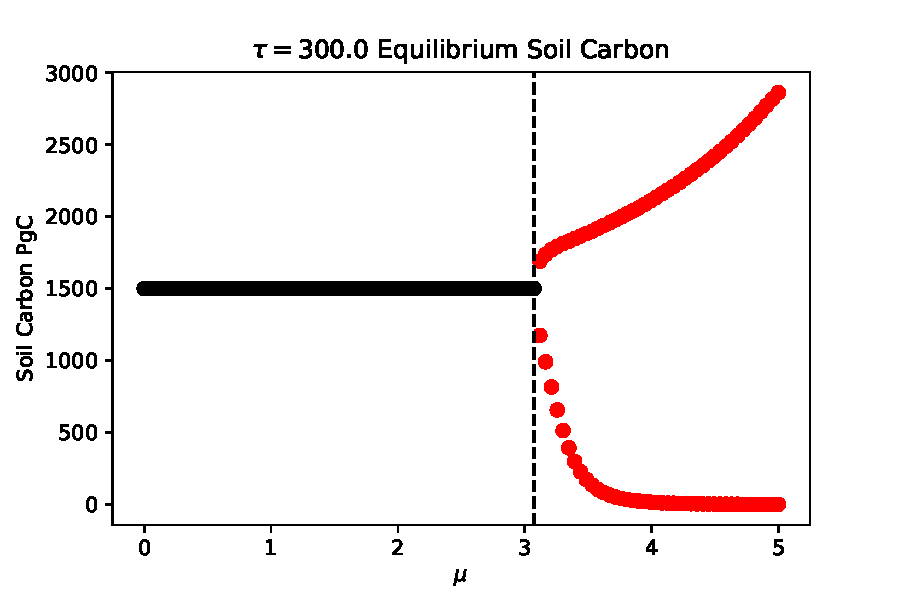
\includegraphics[keepaspectratio,width=\textwidth]{one_box_model_soil_carbon_equilibrium_tau_300.0}
  \caption{Equilibrium Soil Carbon for a one box model as a function of $\mu$ with a slow ocean response.}
  \label{fig:slow_response_bf_diagram}
\end{figure}
For the case where $\tau = \SI{300}{\year}$ I integrate \cref{eq:one_box_ocean} so numerically find the equilibrium as a function of $\mu$, which I plot in \cref{fig:slow_response_bf_diagram}.
Where there is an oscillatory response I plot the maximum and minimum in red. It can be seen that the agreement with the numerics is good.


\section{Two Box Model}
To improve the realism of the model, I will now consider the two box ocean case. In order to do this \cref{eq:one_box_ocean} must be modified to include
two ocean stores of carbon $C_1$ and $C_2$. Each box will have their own timescale $\tau$ and $\tau/\epsilon$ respectively. This notation is suggestive of
$C_1$ being a fast box and $C_2$ being a slow box, although this restriction is not necessary.

This leads to the following system of equations:
\begin{subequations}
  \begin{align}
    \label{eq:two_box_ocean}
    \dv{C_s}{t} &= \Pi(C_a) - r_0 C_s \left(\frac{C_a}{C_{a0}}\right)^{\mu} \\
    \dv{C_1}{t} &= fk(C_a - C_{a0}) - \frac{C_1}{\tau} \\
    \dv{C_2}{t} &= (1-f)k(C_a-C_{a0}) - \epsilon\frac{C_2}{\tau} \\
    C_a &= \mathcal{C} - C_s - C_1 - C_2.
  \end{align}
\end{subequations}
Again note the equilibrium at $C_a = C_{a0}$,$C_s = C_{s0}$ and $C_1 = C_2 = 0$. To determine the stability of this state the eigenvalues of the Jacobian
of \cref{eq:two_box_ocean} must be computed, which involves finding the roots of a cubic characteristic polynomial.
Whilst this is possible in principle it is analytically very challenging.

To avoid this therefore I will give some heuristic arguments as to why a Hopf bifurcation occurs at a critical value of $\mu$. I will then solve a special case
of the characteristic polynomial of the Jacobian, which corresponds to assuming the existence of a Hopf bifurcation. Under this assumption I find
critical values of $\mu$ at which a Hopf bifurcation could occur, which I then verify with a numerical investigation.

\subsection{A Heuristic Argument}
For this section, the assumption of a timescale separation in ocean responses will be assumed, namely that $\epsilon \ll 1$. It has already been shown that a long timescale
single ocean box will lead to a Hopf so it is reasonable to expect that adding a faster box will not change this. Here I give a more mechanistic argument.

Due to the timescale
separation, over short timescales the slow box can be ignored and so it will behave like a one box system. As a result, it can be expected that there
is a value of $\mu$ which leads to an instability. This instability leads to a high atmospheric carbon state, but the ultimate fate of this carbon will depend on the long-time response of the oceans, in other
words on the slow box. Over these longer timescales we can treat the system as a one box model with the ocean box corresponding to the slow box.
Over these long timescales the slow ocean box will absorb the excess carbon from the atmosphere which will tend to cool the globe. As a result
the soil can once again become a sink of carbon. However eventually the soil will contain $C_{s0}$ of soil carbon, but it has already been argued that this state is unstable
and so the cycle will start again.

\subsection{Computation of Bifurcation Point}
If the assumption that there is a Hopf bifurcation can be made, then there is another mode of attack. At the Hopf bifurcation a pair of complex conjugate eigenvalues
cross the imaginary axis from the negative real part side to the positive real part side. This means that at the bifurcation, the eigenvalues are purely imaginary. It is
comparatively easy to solve a cubic equation under the assumption of imaginary roots.

The characteristic polynomial of the Jacobian of \cref{eq:two_box_ocean} will be of the form
\begin{equation}
  \label{eq:generic_cubic}
  \gamma^3 + a_1 \gamma^2 + a_2 \gamma + a_3 = 0,
\end{equation}
where $\gamma$ is an eigenvalue. As has been stated, at the Hopf bifurcation, $\gamma$ is purely imaginary so the substitution $\gamma = i\lambda$ with $\lambda \in \mathbb{R}$
can be made. Then \cref{eq:generic_cubic} becomes
\begin{equation}
  \label{eq:cubic_with_imaginary_root}
  -i\lambda^3 - a_1 \lambda^2 + i a_2 \lambda + a_3 = 0. 
\end{equation}
For this equation to be satisfied, both real and imaginary parts of \cref{eq:cubic_with_imaginary_root} must be zero. This leads to
$\lambda = \pm \sqrt{a_3/a_1}$ and $\lambda = \pm \sqrt{a_2}$. For consistency, these expressions for $\lambda$ must be equal. This requires that $a_3 = a_1a_2$.
Alternatively, both expressions for $\lambda$ can be satisfied if $a_2 = a_3 = 0$. However, this leads to $\gamma = 0$ which has no non-zero imaginary part and so cannot lead to
oscillatory solutions and thus is not consistent with the assumption that there is a Hopf bifurcation.

The condition $a_1a_2=a_3$  can now be solved for $\mu$. Doing this gives two solutions.
\begin{equation}
  \label{eq:mu_two_box}
  \begin{split}
  \mu^* = &\frac{C_{a0}}{2 \Pi_0 \tau  (1+\epsilon)}
  \Biggl(
  -f k \tau  (1-\epsilon)+r_0 \tau  (2 + k \tau +2 \epsilon)+k \tau  (2+\epsilon)+(1+\epsilon) (1+2 \Pi' \tau +\epsilon)\\
  &\pm\sqrt{
    \begin{split}
    f^2 k^2 \tau ^2 (1-\epsilon)^2-&2 f k \tau  (1-\epsilon) \left(r_0 \tau  (k \tau +2 \epsilon +2)-k \tau  \epsilon -(1+\epsilon)^2\right)\\+
    \left(1+k r_0 \tau ^2-k \tau  \epsilon -\epsilon ^2\right)^2
  \end{split}}
  \Biggr)
  \end{split}.
\end{equation}
This equation is very unwieldy but in the case of a timescale separation where $\epsilon \ll 1$, a zeroth order approximation for \cref{eq:mu_two_box} can be derived. It is given by
\begin{equation}
  \label{eq:mu_two_box_zero_eps}
  \begin{split}
  \mu^* \sim &\frac{C_{a0}}{\Pi_0}\Biggl(
    \frac{1}{2\tau} + k(1 - \frac{1}{2}f + \frac{1}{2}r_0 \tau) + r_0 + \Pi'\\
    &\pm\frac{1}{2}\sqrt{\frac{1}{\tau^2} + \frac{2kf}{\tau} + k(kf^2 + 2 (1 - 2f)r_0  - 2 k r_0\tau f  + k r_0^2 \tau^2)}\,\Biggr)
\end{split}
\end{equation}
as $\epsilon \rightarrow 0$.
Note that there are 2 values of $\mu$ that satisfy the consistency condition and so there could be two Hopf bifurcations. It can be further noted that
in the case where $\epsilon = 1$ and $f=1$ then \cref{eq:mu_two_box} should reduce to the one box condition.
Performing this analysis gives
\begin{equation}
  \label{eq:mu_zero_one}
  \mu^*_{\pm} = \frac{C_{a0} \left(\pm\left(-k r_0 \tau ^2+k \tau +1\right)+r_0 \tau  (k \tau +2)+k \tau +2 \Pi' \tau +1\right)}{2 \Pi_0 \tau}
\end{equation}
or
\begin{align}
  \label{eq:mu_zero_one_cases}
  \mu_+^* &= \frac{C_{a0}}{C_{s0}} + \frac{C_{a0}}{\Pi_0}\dv{\Pi}{C_a} + \frac{C_{a0}}{C_{s0}} \left(\frac{k}{r_0} + \frac{\tau^{-1}}{r_0}\right) \\
  \mu_-^* &= \frac{C_{a0}}{C_{s0}} + \frac{C_{a0}}{\Pi_0}\dv{\Pi}{C_a} + \frac{C_{a0}}{C_{s0}}k\tau 
\end{align}
which correspond does indeed correspond to the conditions (\cref{eq:instability_condition_one_box_fast,eq:instability_condition_one_box_slow}) derived for the one box case.

\subsection{Numerical Results}
To test if the value of $\mu$ in \cref{eq:mu_two_box} does correspond to a Hopf bifurcation, I integrate \cref{eq:two_box_ocean} with $f = 0.5$, $\tau = 0.45$ and $\epsilon = 0.004$.
Furthermore I numerically compute the eigenvalues of the Jacobian for a range of values of $\mu$. The eigenvalues of the Jacobian are plotted in \cref{fig:eigen_values_of_the_jacobian},
which show the eigenvalues cross the imaginary axis at the predicted bifurcation point, $\mu_-$.
\begin{figure}
  \centering
  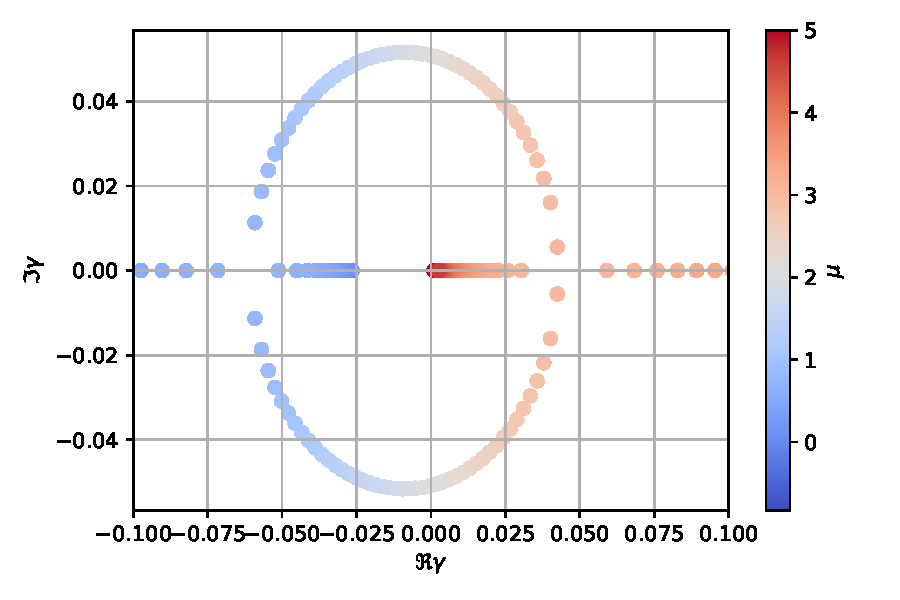
\includegraphics[width=\textwidth,keepaspectratio]{complex_plane_two_box_eig}
  \caption{The eigenvalues of the two box Jacobian plotted in the complex plane. The colours correspond to the value of $\mu$. The colour scheme is chosen so that the colours change at $\mu = \mu_-$ }
  \label{fig:eigen_values_of_the_jacobian}
\end{figure}
\begin{figure}
  \centering
  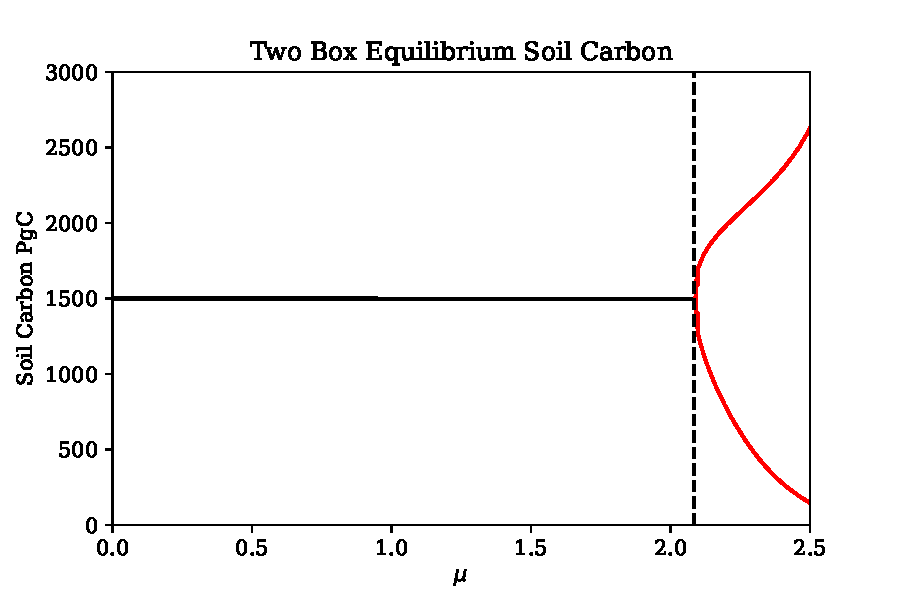
\includegraphics[keepaspectratio,width=\textwidth]{two_box_model_soil_carbon_equilibrium}
  \caption{The equilibrium values of soil carbon for the two box model. Where the equilibrium state is oscillatory, the minimum and maximum are plotted in red}
  \label{fig:two_box_bf_diagram}
\end{figure}
Furthermore, the equilibrium soil carbon state is plotted in \cref{fig:two_box_bf_diagram}. It can be seen that the bifurcation corresponds to the theoretical prediction.
In all my integrations, there did not appear to be a bifurcation at $\mu_+$. This could be because $\mu_+$ represents a spurious solution. Alternatively there could be other
parameters for which $\mu_+$ represents a real bifurcation. In any case as $\mu_+ > \mu_-$, the bifurcation at $\mu_-$ will have more relevance to the climate system.

\section{Model Comparison}
In this section, I have introduced 3 models for the Earth's carbon cycle: a one-box, a two-box and a more complex model. Each model suggests the carbon cycle
has bifurcations for large enough values of a sensitivity. In this next figure, \cref{fig:imogen_one_box_two_box} I plot the equilibria for each model.
\begin{figure}
  \centering
  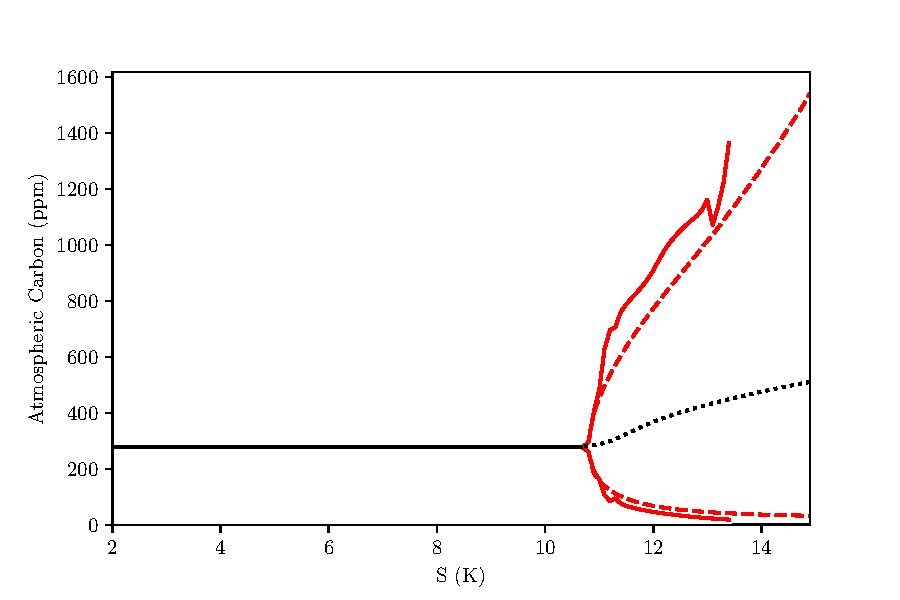
\includegraphics[keepaspectratio,width=\textwidth]{imogen_one_box_two_box}
  \caption{A comparison of bifurcation diagrams across the models. Dots refer to IMOGEN, the ``+'' refers to the one box model and ``$\times$'' to the two box.
  Equilibria are plotted in black and the minimum and maximum of any oscillations are in red.}
\label{fig:imogen_one_box_two_box}
\end{figure}
I have chosen the ocean parameters so that the bifurcation points line up. For the one box model, this involved setting $\tau = \SI{2.34}{\year}$. For the two box model there
was more freedom in the parameter choice. I set $\tau_1 = \SI{0.1}{\year}$, $f = 0.92$ and $\epsilon = 1.6\times 10^{-5}$.

Unlike the other two models, the one box model does not give any oscillatory behaviour. The two box model gives  oscillations for all values of $S$ above a threshold, whereas IMOGEN shuts the
oscillations down at large enough $S$, and no carbon is found in the atmosphere. However the two box model and IMOGEN give qualitative agreement on the amplitude of the limit cycles beyond the bifurcation
point.

\section{Conclusion}
In this chapter I have taken a simple but but realistic model of the carbon cycle and shown that only certain parameter values are compatible with the qualitiative behaviour
of terrestrial carbon cycle since during the holocene. In particular these parameters relate to key sensitivites in the Earth system: the climate sensitivity, the sensitivity of
terrestrial carbon to temperature and the sensitivites of net primary production to \ce{CO2}. In this model I find that the negative feedbacks on the system (namely changes in net primary
production due to increased \ce{CO2}) must be sufficently strong enough to offset the positive feedbacks (the Jenkinson effect).

Although the model was relatively simple, the ocean component is still too complex to handle analytically. I simplified the ocean model down to a box model of the oceans,
which meant I could derive exact results about the bifurcation. I found that a single box could recreate the osciallatory behaviour seen for large enough climate senitivites,
however it did not do this at the correct bifurcation point. On the other hand, a two box model could reproduce the oscillations at the correct bifurcation point.

I could then fit the box models to the observed carbon uptake by the oceans to estimate what parameters best fit the observations. These parameters are similar to those found in the more
complex model, although they disagree on the position of the bifurcation.